\documentclass[../../../Bachelorarbeit.tex]{subfiles}
\begin{document}

\subsection{Implementationsphase}
In diesem Unterkapitel findet sich die Dokumentation der Implementation sämtlicher Modelle aus der Projektierungsphase wieder. Zunächst wird im \autoref{Hardwareimp} die Montage der Laboranlage kurz dargestellt. Dazu wird aus der Konfiguratorskizze unter Berüchsichtigung der Maße des Laborraumes und der entsprechenden Anforderungen an den Aufbau des Positioniersystems die Anlage aufgebaut. Nachdem alle Gehäuseelemente an der Wand und dem Boden verankert sind können die Steuerungskomponenten, die Aktuatoren und die Sensoren an diesen befestigt werden. Weiterhin umfasst der nachfolgende Abschnitt die Verdrahtung der elektrischen Komponenten nach entwickeltem Stromlaufplan und der Netzwerkdarstellung aus dem \autoref{Stromlaufplan}.\\
Im zweiten Unterabschnitt (\autoref{Softwareimp}) wird die Implementation der modellierten Diagramme zur Steuerungssoftware vorgenommen. Da durch die Wahl der Steuerung (Logic Motion Controller von Schneider Electric), wie bereits in der Anforderungsanalyse festgestellt, die Umgebung zur Programmierung der Systemsoftware festgelegt ist, besteht die Möglichkeit Templates aus dieser zu nutzen, welche den Softwareentwicklungsprozess vereinfachen. Der Unterabschnitt zur Software-Implementation behandelt somit die schrittweise Darstellung der Umsetzung der Automatisierungssoftware aus dem von Schneider Electric bereitgestellten \textit{Motion Template Full}.

\subsubsection{Hardware-Implementation} \label{Hardwareimp}
Für die Umsetzung der Hardware wird die Kofiguratorgrafik aus der Konzeptphase wird aufgegriffen und gilt als Grundlage für die reale Umsetzung der Hardwarebereiche des Systems. Da im Konfigurator bereits die Kernanforderungen an die Systemhardware berücksichtigt wurden, müssen beim Bau und der Montage des Gehäuses \bzw des Anlagengerüsts nur noch die nicht-funktionalen Anforderungen an dieses und den umliegenden Raum berücksichtigt werden.\\
Durch die Form und die Ausmaße des Laborraumes ergibt sich eine maximale Höhe des Gehäuses von 2230\si{\mm}. Die horizontale Ausdehnung der Anlage wird nicht durch den Raum begrenzt. Die Entscheidung wurde auf Grund von Subjektiven Anschaulichkeitskriterien getroffen. Resultat ist eine horizontale Ausdehnung der x-Achse von 2000\si{\mm}, was ungefähr der Gangbreite im Laborraum entspricht. Folglich ist der bewegliche Teil des Positioniersystems mittig zum Durchgang im Raum ausgerichtet. Sowohl rechts als auch links neben der Positioniereinheit ist ein bereich von jeweils 600\si{\mm} reserviert, in dem Ablagepositionen an der Wand befestigt weren können. Die rechte Seite der Anlagenkonstruktion besitzt zusätzlich noch ein weiteres Aluminium Profil, welches später benötigt wird, um den Schaltschrank und die Steuerungshardware am System zu fixieren. Nachfolgende Grafik zeigt das an der Laborraumwand montierte Anlagengerüst, an welches im nächsten Schritt die Steuerungshardware befestigt wird.

\begin{figure}[H]
    \centering
    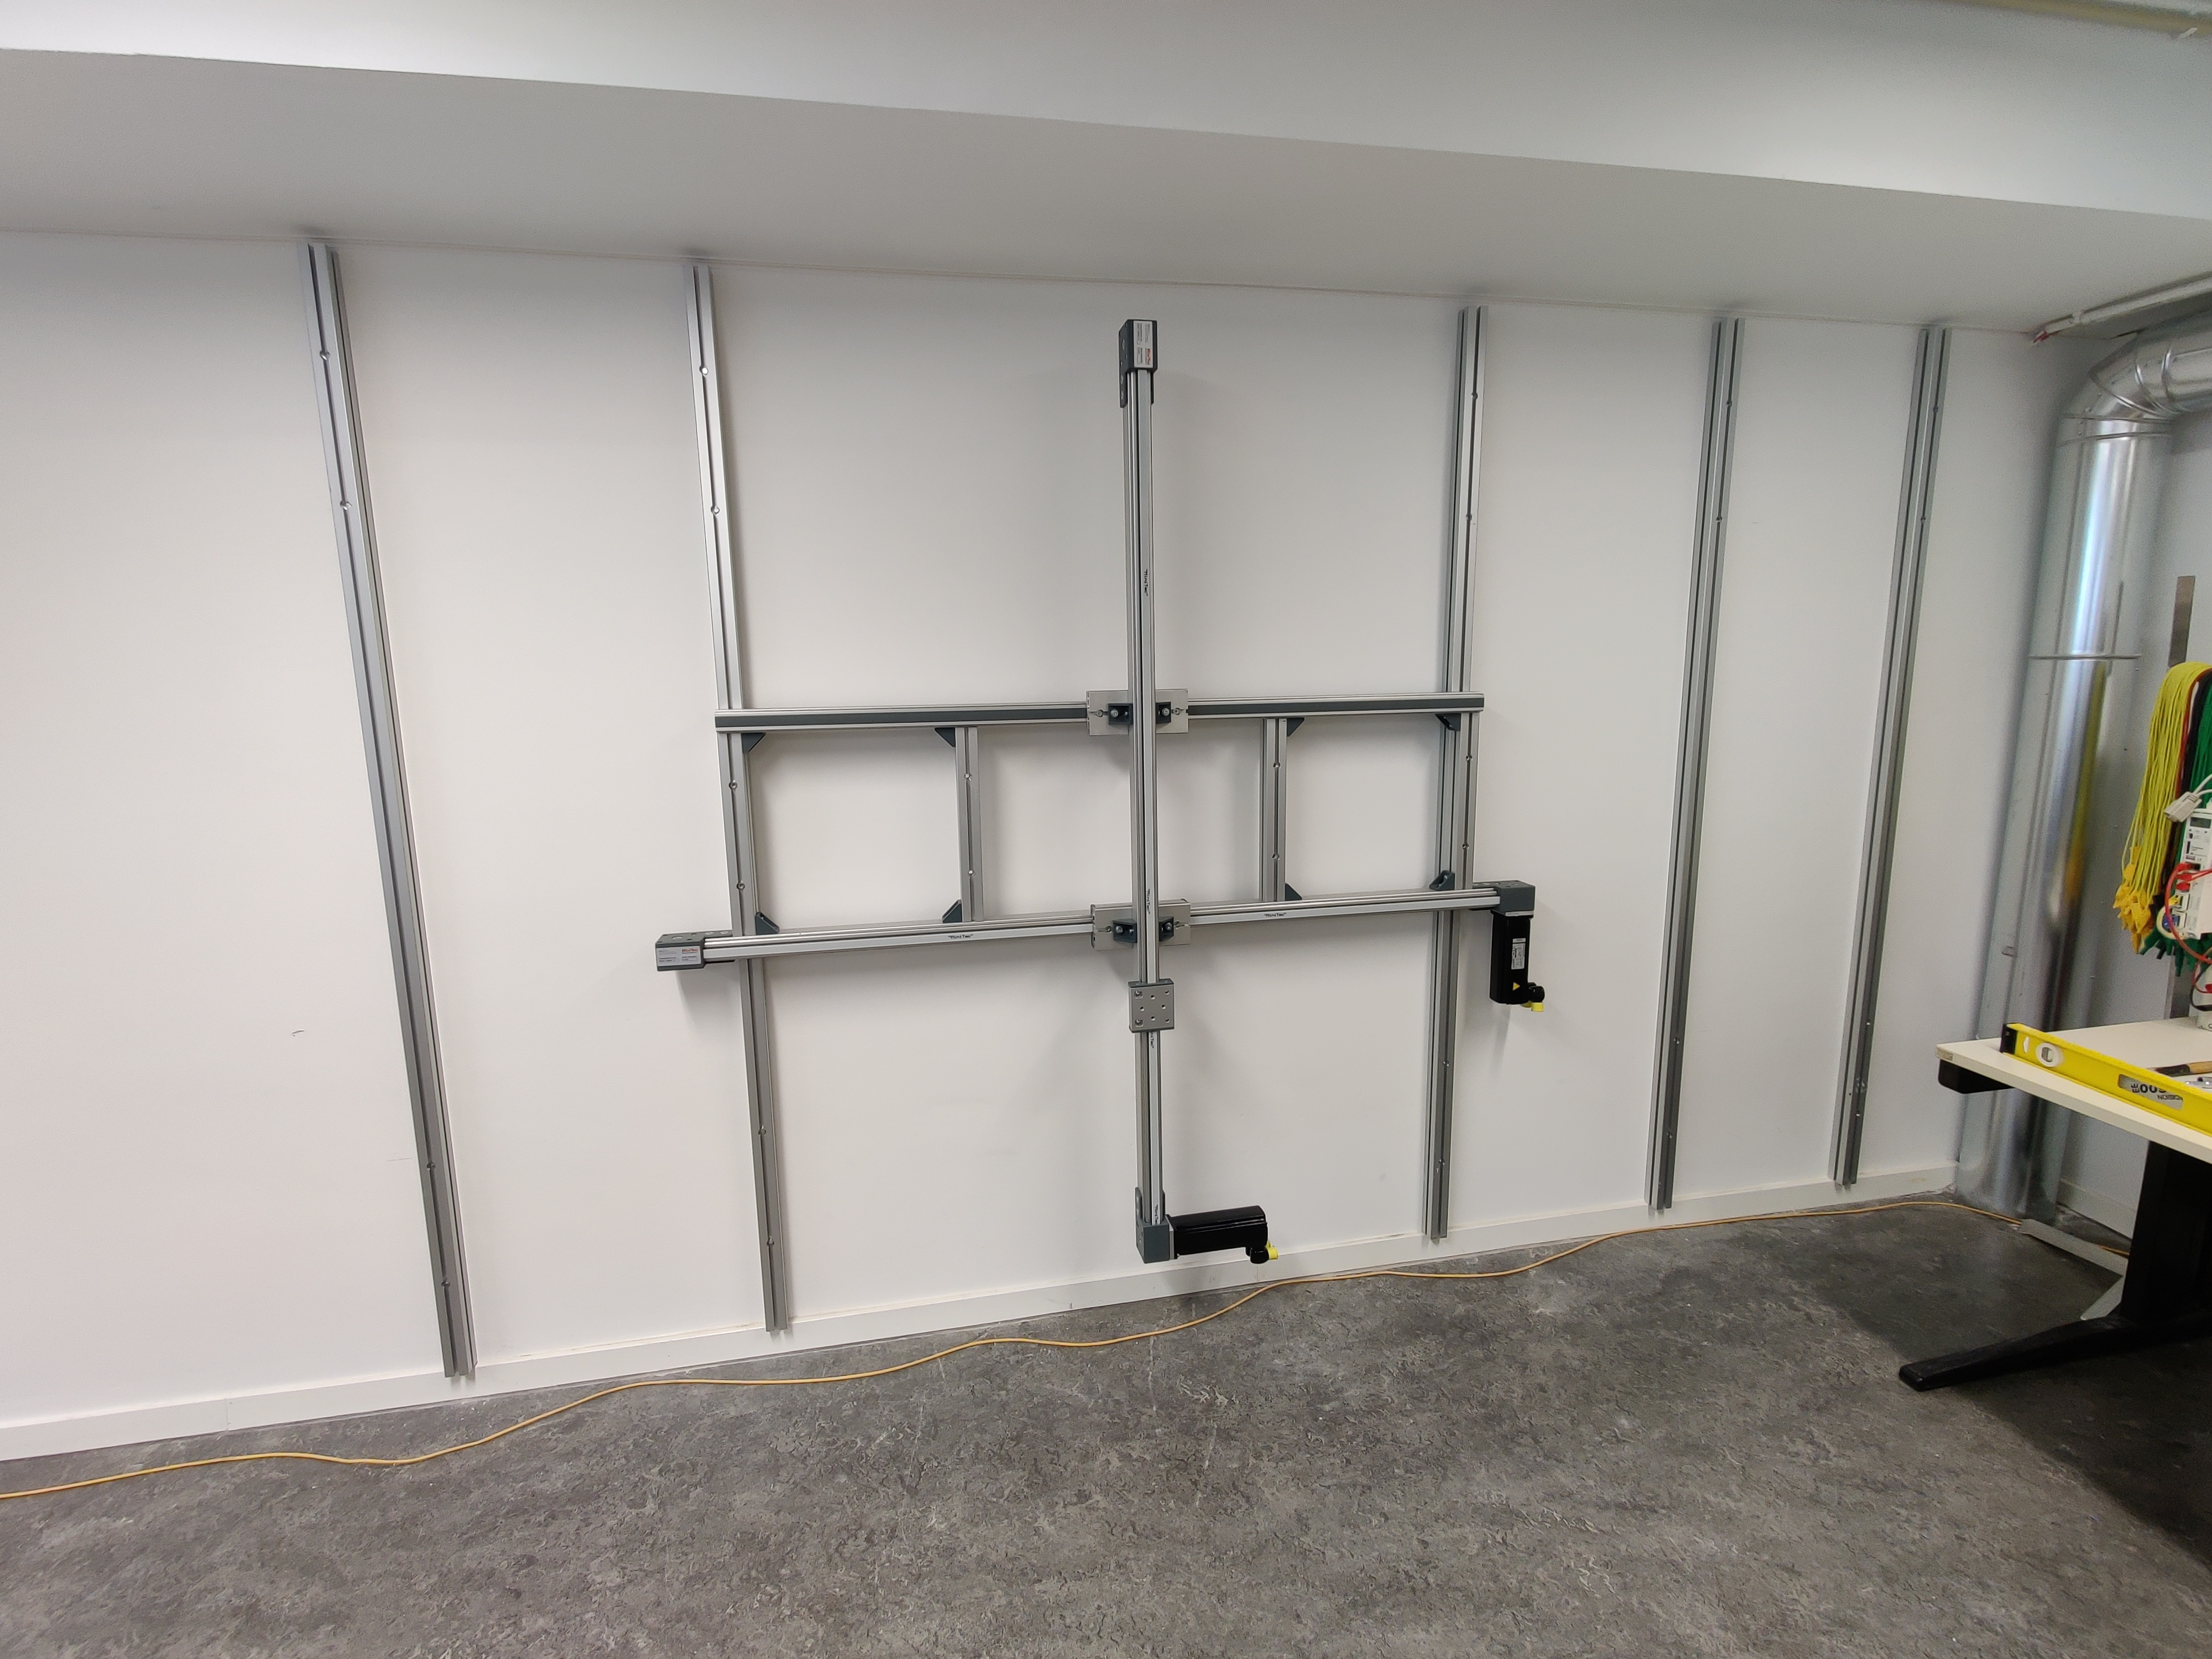
\includegraphics[width=0.7\textwidth]{Images/Anlagengeruest.jpg}
    \caption[Anlagengerüst]{Anlagengerüst des Gehäuses vom mehrachsigen Positioniersystem an der hinteren Laborwand im Raum G 422}
    \label{fig:my-img20}
\end{figure}

Im nächsten Schritt der Hardware-Implementation werden die Steuerung (LMC400) das Netzgerät (LXM 62P) und der Servoregler (LXM 62D) an Querverstrebungen der beiden rechten Profile verschraubt. Es gilt die Montageanleitung zu beachten. % Quelle hinzufügen

\begin{figure}[H]
    \centering
    \begin{subfigure}[c]{0.42\textwidth}
        \centering
        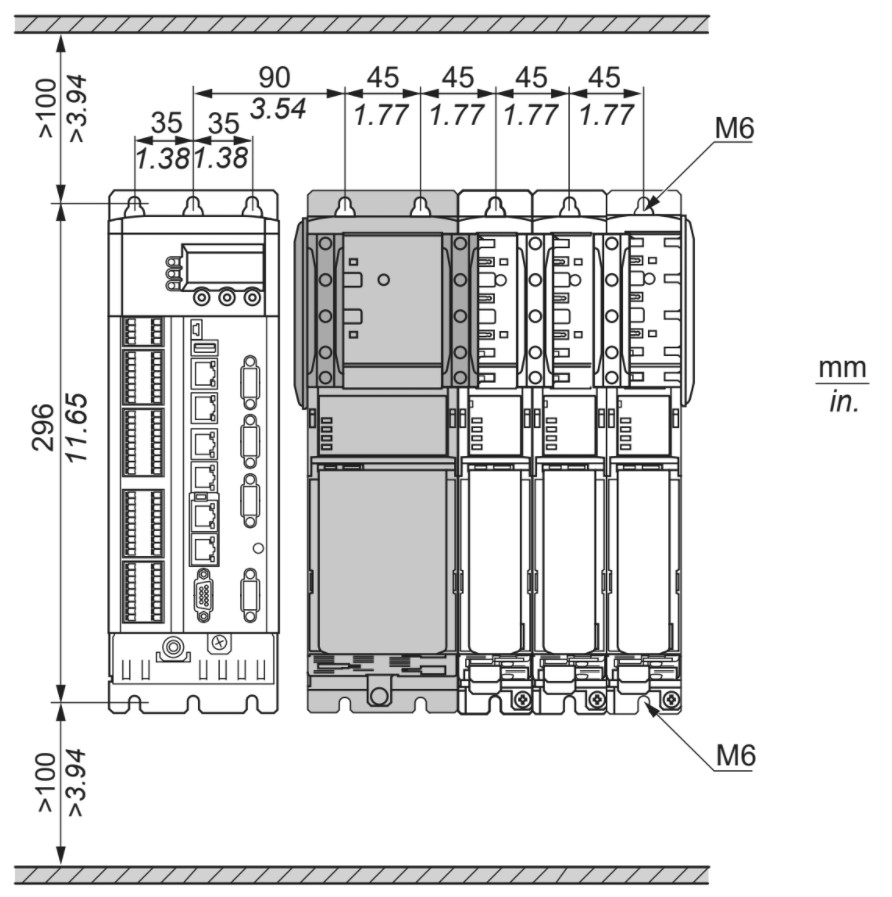
\includegraphics[width=0.9\textwidth]{Images/Steuerungshardwareinstallation.jpg}
    \end{subfigure}
    \begin{subfigure}[c]{0.42\textwidth}
        \centering
        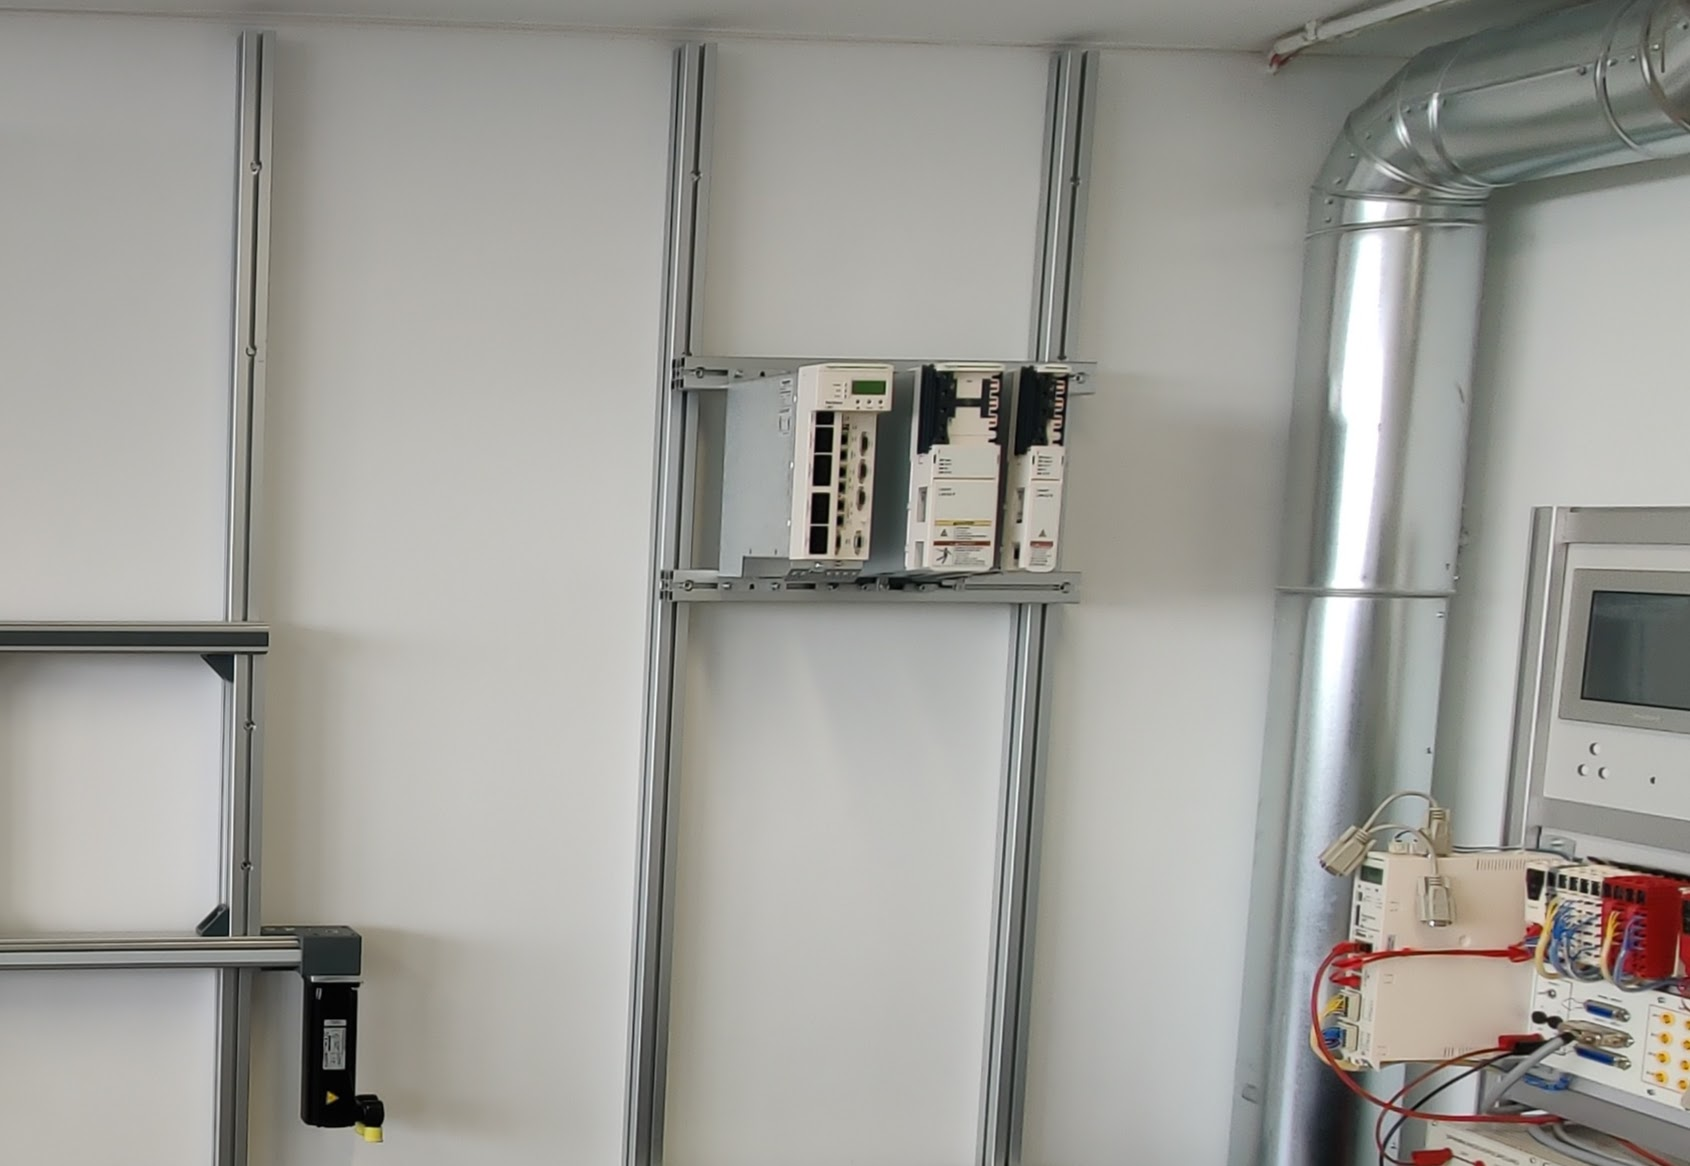
\includegraphics[width=0.9\textwidth]{Images/Steuerungshardware.jpg}
    \end{subfigure}
    \caption[Steuerungsinstallation]{Installation der Steuerungshardware am Gehäuseaufbau des Positioniersystems}
    \label{fig:my-img21}
\end{figure}

Bevor die in der Konfiguratorskizze aufgeführten Sensoren und Aktuatoren verbaut werden können, sind noch weitere Profile notwendig, um den Gehäusebau zu komplettieren. 500\si{\mm} von der Wand entfernt auf Höhe der äußeren Profile des Positionierbereiches werden zwei senkrechte Aluminiumstempel an Decke und Boden befestigt. Diese sind das vordere Ende des mehrachsigen Positioniersystems. Das Gehäusegerüst ist nun vollständig und umschließt den Berech, in dem Positionieraufgaben durchgeführt werden können mit der Laboranlage.\\
Zwischen den beiden linken Profilen und den beiden rechten Profilen werden Plexiglasscheiben angebracht, die das Hineingreifen in den Fahrbereich der Anlage von den Seiten verhindern sollen. An der Front wird ein Lichtvorhang bestehend aus Emitter und Receiver montiert. Dieser befindet sich auf der Innenseite an den zuletzt angebauten senkrechten Stempeln. Der Lichtvorhang dient ebenso wie die Plexiglasscheiben zum Schutz von Leib und Leben. Im Gegensatz zu den Scheiben erlaubt der Lichtvorhang jedoch im unbewegten Zustand des Systems das Eindringen von Personen in des Arbeitsbereich.\\
Folgende Grafik zeigt zu den soeben genannten Komponenten zusätzlich noch die in den Anforderungsanalyse ermittelten vier Endlagesensoren, die Servomotoren für x- und z-Achse, sowie E-Ketten zu den beweglichen Achsen.

\begin{figure}[H]
    \centering
    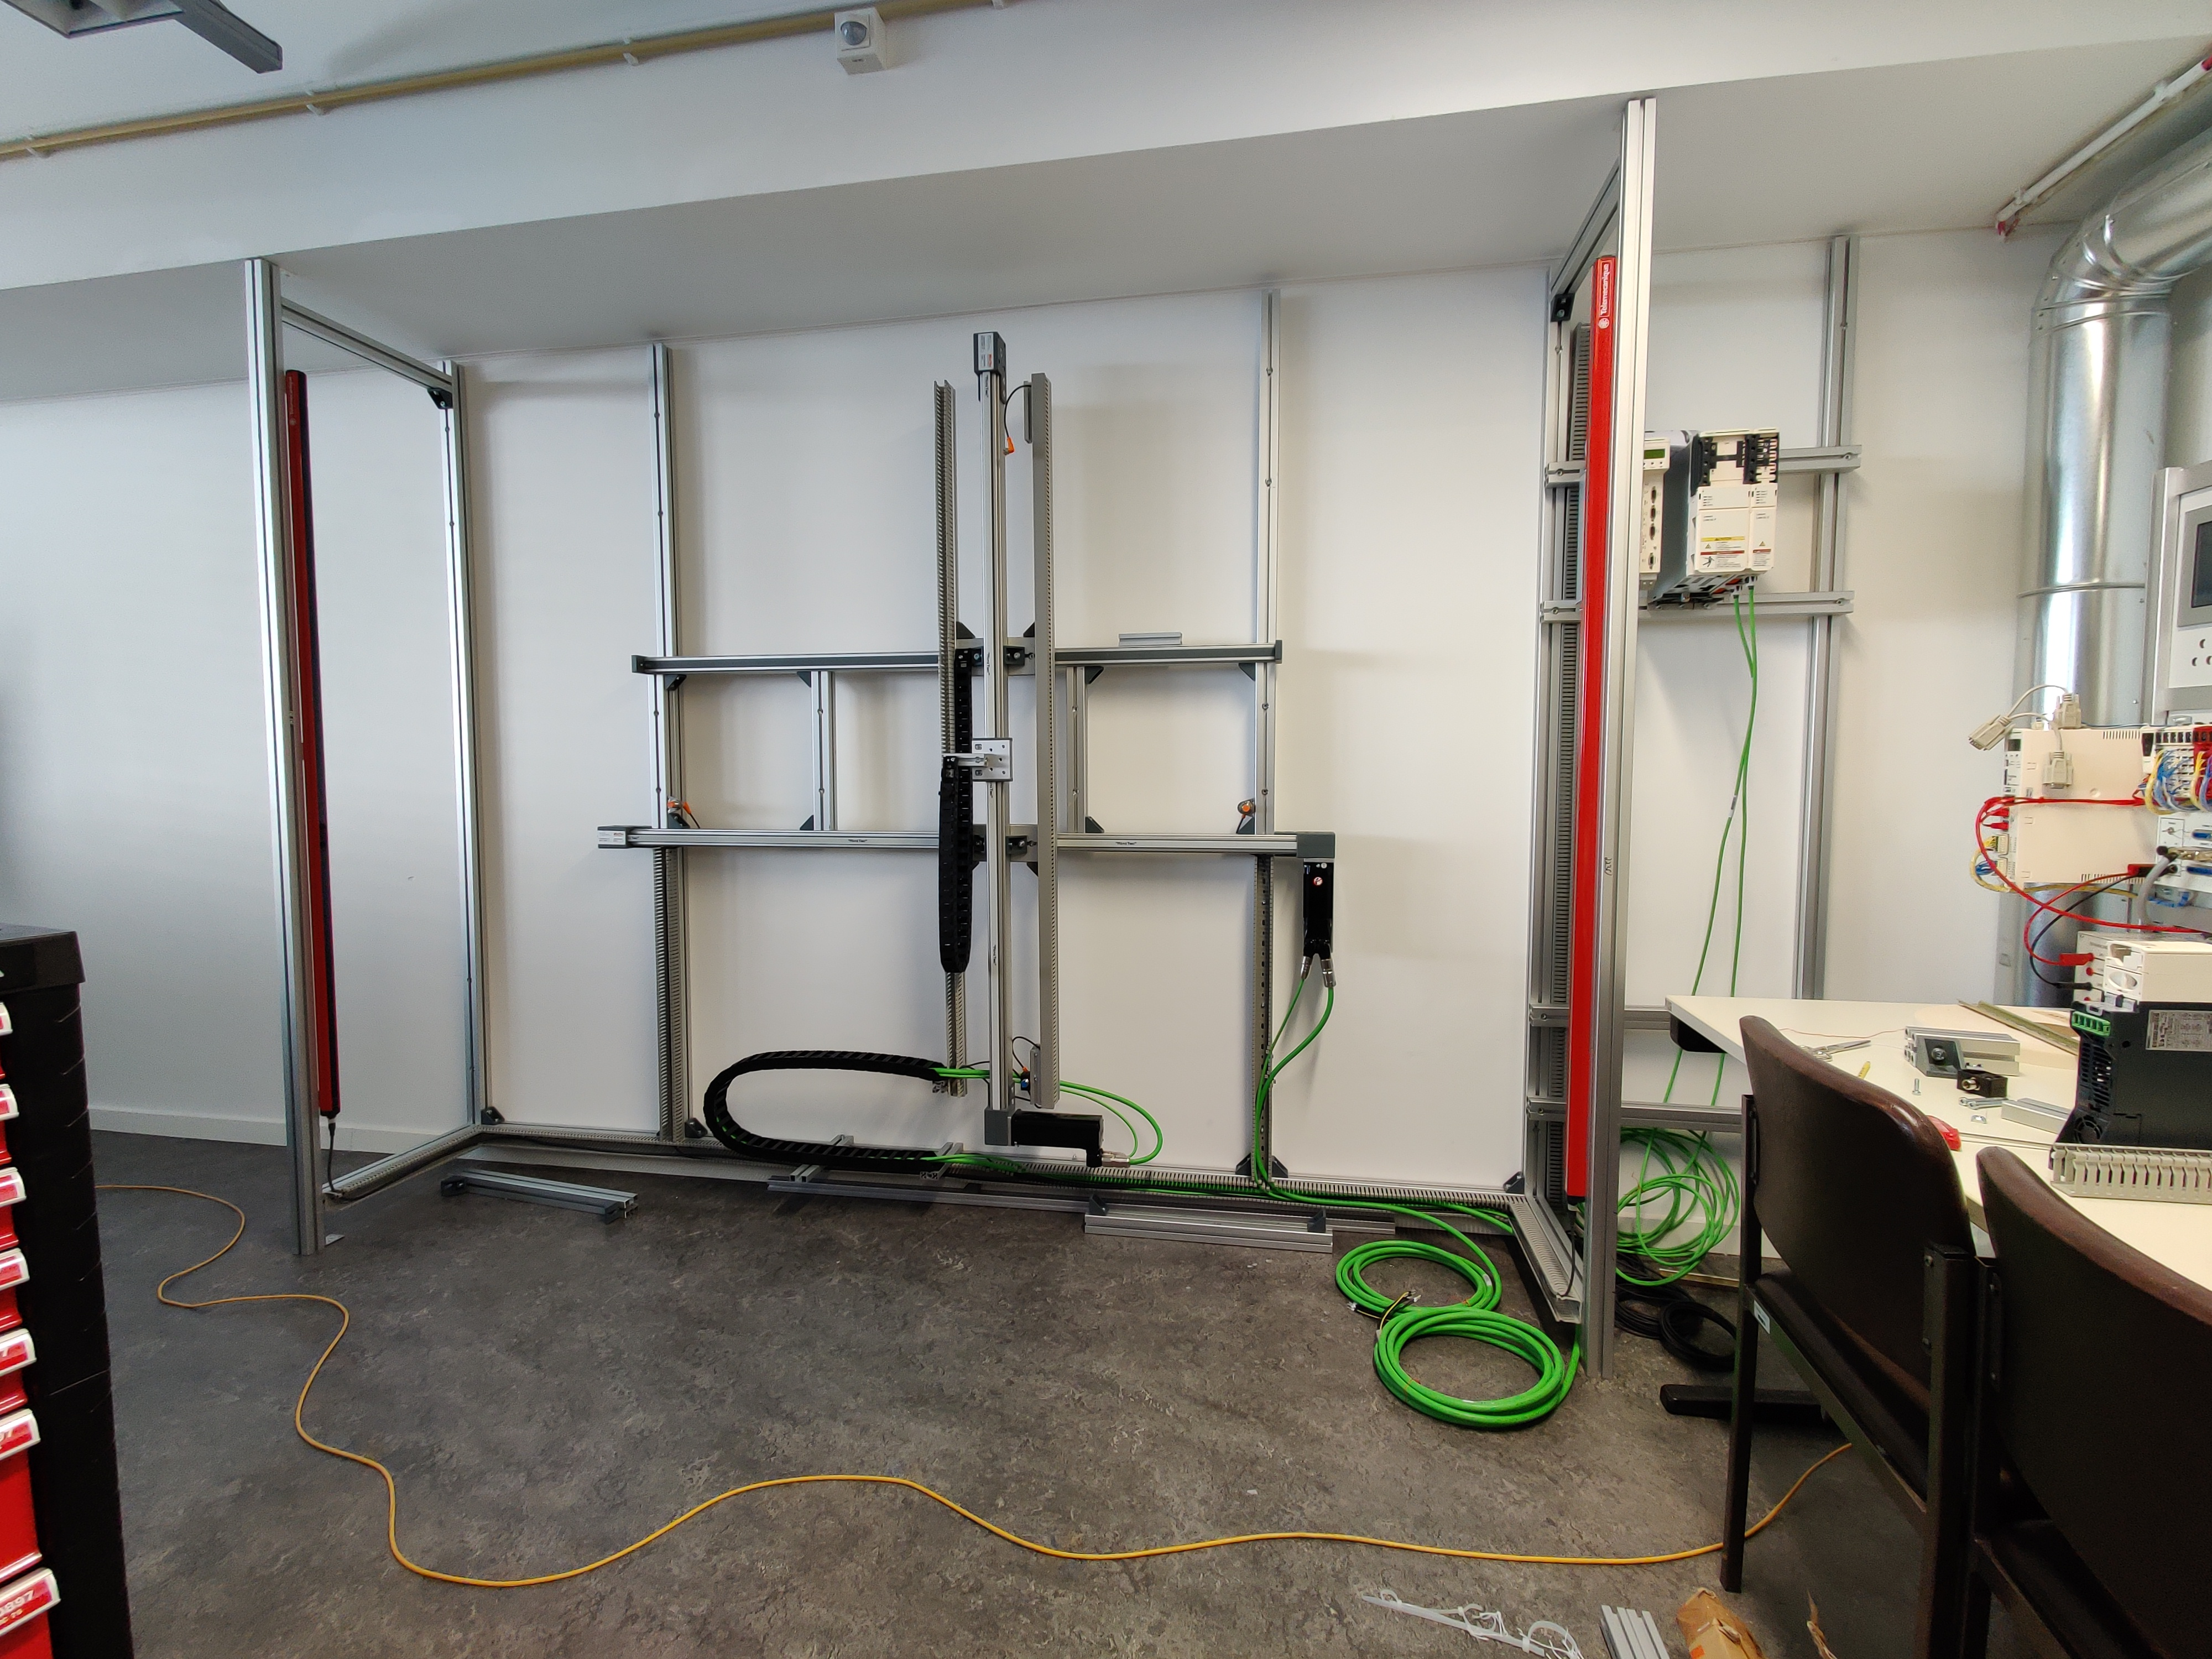
\includegraphics[width=0.7\textwidth]{Images/AktuatorenSensoren.jpg}
    \caption[Aktuator- und Sensorinstallation]{Installation von Sensoren und Aktuatoren des mehrachsigen Positioniersystems}
    \label{fig:my-img22}
\end{figure}

Der Schaltschrankeinbau und die Verdrahtung des Systems stellt den letzten Schritt in der Hardware-Implementierung dar. Als Schaltschrank wurde ein Modell der Firma Rittal gewählt. Die Breite des Schrankes ist durch den gewählten Aufbau bereits festgelegt und beträgt 600\si{\mm}. Aufgrund der Anzahl der Klemmen und dem Wunsch \acs{ea}-Module sowie weitere Steuerungskomponenten physisch von normalen Klemmen zu trennen, wurde entschieden eine Schaltschrankkonfiguration zu wählen, die in der Höhe zwei Hutschienen unterbringt. Die gewählte Schrankhöhe liegt deswegen bei 380\si{\mm}. Zuletzt muss die Tiefe des Schaltschranks ausreichend sein, um die tiefste Komponente, die im Schaltschrank verbaut werden soll, unterbringen zu können. Da bereits die kleinste verfügbare Variante des gewählten Schrankes diese Anforderung erfüllt, hat der zu verbauende Schaltschrank eine Tiefe von 210\si{\mm}.\\
Wie bereits angedeutet ist in der Grafik unten zu erkennen, dass die untere der beiden Hutschienen sämtliche Klemmen beherbergt inklusive der Absicherungen für die jeweilge Spannungsebene, so wie im Stromlaufplan geplant. An der Oberen Hutschiene befinden sich die Modicon TM5 \acs{ea}-Module, die als Erweiterung für die Ein- und Ausgänge des \acs{lmc} dienen. Die im Bild als rot gefärbte Komponente zu erkennende Steuerung, ist der Safety Logic Controller, der für die Berechnung der Sicherheitsfunktionen des Systems verantwortlich ist. Dazu besitzt dieser jeweils vier digitale Ein- und Ausgänge.\\
Rechts daneben auf der selben Schiene ist die Wago PFC 200 Steuerunge angebracht, welche mit Hilfe ihrer Energieklemme die Leistungsaufnahme des Systems messen soll.\\
Ganz Rechts auf der Hutschiene ist ein Ethernetswitch montiert, an welchen beide Steuerungen (LMC400 und Wago PFC 200) per Ethernetkabel angeschlossen sind. Durch den Einsatz des Switches führt nach Vertigstellung der verdrahtung nur ein Kabel zur Programmierung der beiden Steuerungen aus dem Schaltschrank heraus.\\
Weiterhin ist auf der rechten Schrankwand der Hauptschalter platziert. Über dieser aktiviert oder deaktiviert die Stromversorgung des Schaltschrankes und somit auch aller Systemkomponenten.\\
Die Verdrahtung erfolgt nach Stromlaufplan. Dieser beinhaltet auch die Kopplung der einzelnen Module aus der PacDrive3 Serie, die verbaut wurden (LMC400, LXM 62P, LXM 62D, Modicon TM5 Module, Modicon TM5 SLC100 Sicherheitsmodule). 

\begin{figure}[H]
    \centering
    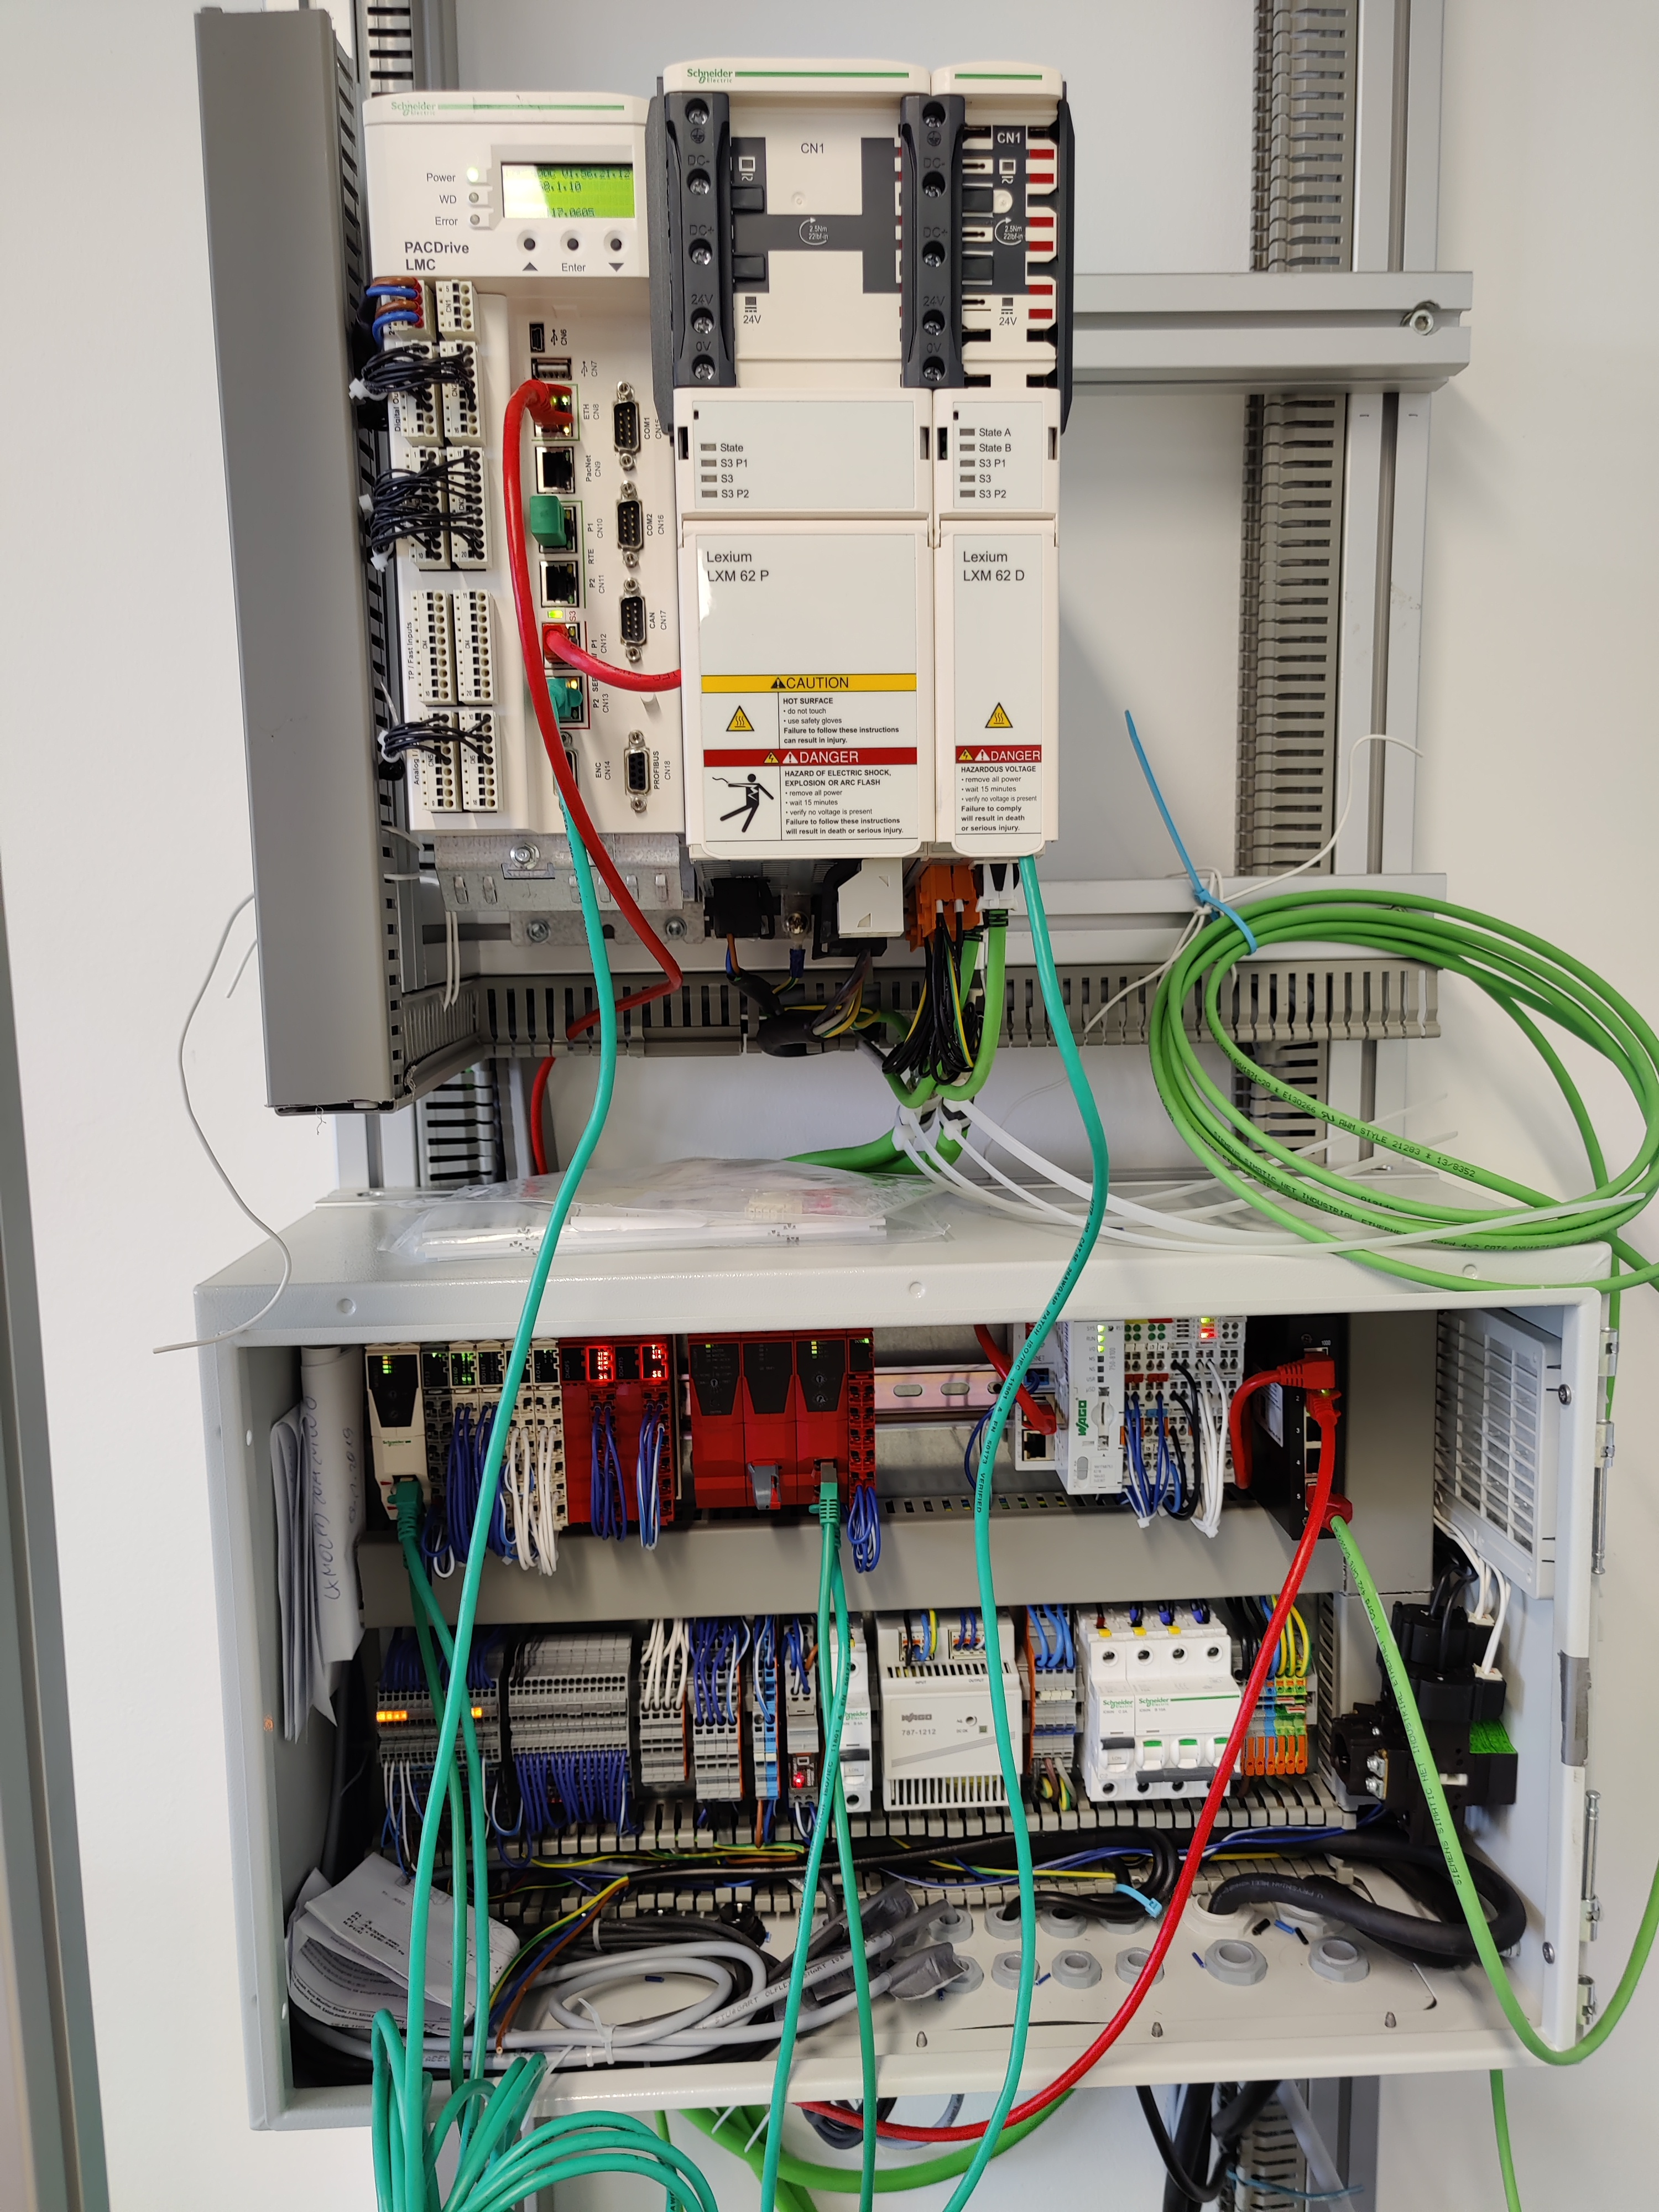
\includegraphics[width=0.66\textwidth]{Images/Schaltschrank.jpg}
    \caption[Schaltschrank]{Einbau und Verdrahtung des Schaltschranks}
    \label{fig:my-img23}
\end{figure}

% Schaltschrankfront Text + Bild !!!

\subsubsection{Software-Implementation} \label{Softwareimp}
In diesem Unterabschnitt wird die Realisierung der Automatisierungssoftware dokumentiert. Grundlegend soll aus der Modellierung der Software im vorhergegangenen Kapitel (Projektierung) das Programm für das mehrachsige Positioniersystem geschrieben werden. Wie bereits in der Einleitung zu diesem Unterkapitel erwähnt, resultiert die Wahl der Steuerungskoponenten, also konkret die Wahl Komponenten aus der PacDrive3 Serie von Schneider Electric auszuwählen, in dem Zwang mit der auf Codesys 3.5 basierten Entwicklungsumgebung Machine Expert zu arbeiten. Diese besitzt bereits mehrere Templateprojekte für verschiedene Anweundungsfälle. Die Firma Schneider Electric empfiehlt die Nutzung des jeweiligen Programmtemplates für den gewünschten Anwendungsfall. Grund dafür ist die Minimierung vom Programmieraufwand. Ziel soll es sein lediglich Konfigurationen an einem Modularen Template vorzunehmen, so dass dieses die eigenen Anforderungen erfüllt. \\
Begründet durch diese Aussagen wird zunächst davon ausgegangen, dass durch die Nutzung des \textit{Motion Template Full} mit überschaubarem Programmier- und Parametrieraufwand die Sammlung der eigenen Anforderungen an das Automatisierungsprogramm und dessen Funktionen erfüllt werden. Dies gilt im anschließenden Unterkapitel in den jeweiligen Testfällen zu bestätigen. \\
Zunächst findet eine schrittweise Auflistung zur Umsetzung der Steuerungssoftware aus dem bereitgestelltem Template statt. Diese unterteilt sich in folgende Vorgehensschritte:

\begin{itemize}
    \item Anlegen des Projektes
    \item Zuweisen der Ein- und Ausgänge der Steuerungen und deren Erweiterungsmodule
    \item Parametrierung und Inbetriebnahme des Servoreglers für die x-Achse
    \item Parametrierung und Inbetriebnahme des Servoreglers für die z-Achse
    \item Parametrierung und Inbetriebnahme des Netzteils
    \item Implementation der funktionalen Sicherheit
\end{itemize}

Für das \textbf{Anlegen des Projektes} wird die Software Machine Expert Logic Builder auf den Rechnern des Labores benötigt. Alternativ kann auch die veraltete Software SoMachine Logic Builder genutzt werden. Soll von jedem PC aus das System Programmiert und zunächst auch gesteuert werden, so muss die Programmiersoftware vorhanden sein. Ist dies der Fall, so muss anschließend wie folgt vorgegangen werden:

\begin{enumerate}
    \item \textit{LogigBuilder} Programm am Laborcomputer starten
    \item Neues Projekt aus Projektvorlage \textit{MotionTemplateFull} für LMC300/400/402/600/800 anlegen
    \item Im Projektbaum oben links Doppelklick auf \textit{LMC\_PacDrive}
    \item Anschließend im Reiter \textit{Steuerungsauswahl} den LMC400c auswählen (vorher sichergehen, dass der Controller eingeschaltet ist, sonst kann dieser nicht gefunden werden)
    \item Im Projektbaum unter \textit{Sercos\_Master (Sercos Master)} alle untergeordneten Geräte markieren und anschließen entfernen
    \item Etwas tiefer im Projektbaum Doppelklick auf \textit{Geräteaddressierung}
    \item Im neu geöffneten Fenster oben rechts den Button \textit{Sercos Scan starten} drücken
    \item Es erscheinen neue tabellarisch angeordnete Einträge in der Mitte des Fensters (Einträge sind rot eingefärbt)
    \item Unten rechts im offenen Fenster auf \textit{Geräteparameter übernehmen} klicken (Alle vorhandenen Einträge sollten die Farbe zu grün wechseln)
    \item Den \textit{IEC Bezeichner} des Powersupplies ändern zu \textit{PSM\_PowerSupply}
    \item Den \textit{IEC Bezeichner} des von Drive A und B ändern zu \textit{DRV\_Slave1} \bzw \textit{DRV\_Slave2}
    \item Oben links im offenen Fenster über Kombobox drei neue LXM62DxS hinzufügen
    \item \textit{IEC Bezeichner} des ersten neuen Eintrages auf \textit{DRV\_Master} ändern (Wichtig: Gerät sollte auf virtuell eingestellt sein)
    \item \textit{IEC Bezeichner} der beiden anderen Einträge ändern zu \textit{DRV\_Slave3} \bzw \textit{DRV\_Slave4} (Wichtig: Geräte sollte auf virtuell eingestellt sein)
\end{enumerate}

% Bild zur Geräteaddressierung hinzufügen

Um die anliegenden Sensor- und Eingabegerätesignale an den SPS Eingängen, sowie die Aktuatoren und Indikatoren an den SPS Ausgängen nutzen zu können, müssen den Hardwareaddressen im Programm Variablen zugewiesen werden (\eng Mapping). Damit alle \acs{ea}-Variablen an einem Ort als auch global im gesamten Programm verfügbar sind, sollte eine Globale Variablenliste angelegt werden, in der alle Variablen eingetragen werden können. Folgendes Bild zeigt die Globale Variablenliste für die Ein- und Ausgänge des mehrachsigen Positioniersystems.\\

%  Bild zur GVL hinzufügen

Nachfolgend wird das Mapping schrittweise für die Ein- und Ausgangsmodule der mit dem LMC verbundenen Modicon TM5 Geräte vorgenommen. Bei den zuzuordnenden Variablen handelt es sich um die im Datenmodell aufgelisteten Variablen. Dieses dient somit als Grundlage für die Zuweisung der Ein- und Ausgänge.



\end{document}